\chapter{The Daemon}
\label{chap:daemon}
This chapter will explain the design and implementation of the daemon of this project. A daemon is a computer program that runs in the background continuously without any input from a user.
\section{Design}
The daemon has a one main job, to activate rules that require action at a specific or recurring time. Right now there is only one such action, \texttt{Add points}, which when activated has to add points to a given users profile. This cannot be done using a normal website because of the time requirement that the points have to be added at the right time. Further things that the daemon should handle could be such things as \texttt{Activate tag} and \texttt{Block tag} if these were added as actions to the rule system. \autoref{fig:daemonflowchart} shows how the flow of the daemon should work. It should check rules every minute if they should activate, and activate those who should, doing the action specified.

\begin{figure}[!h]
	\centering
		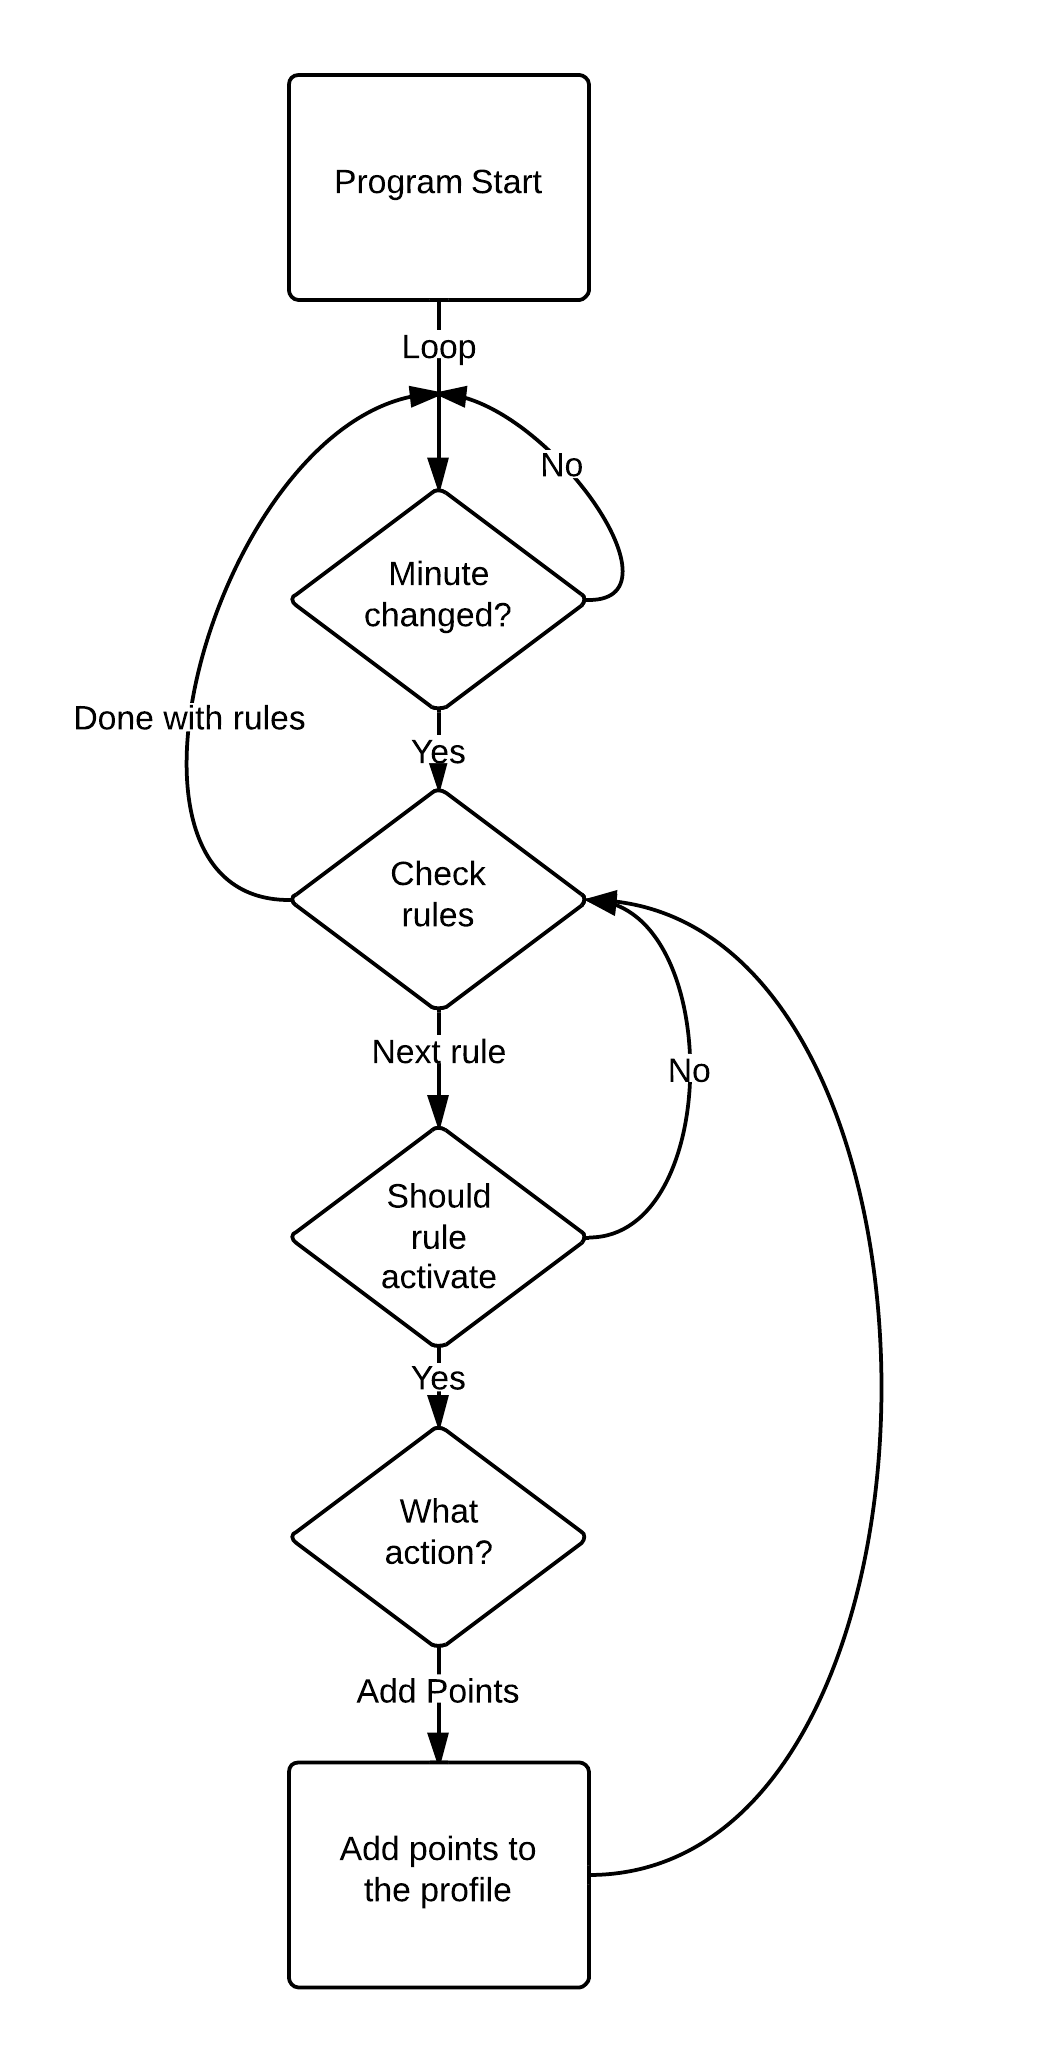
\includegraphics[width=0.65\textwidth]{images/daemonflowchart.png}
	\caption{Flowchart showing how the daemon should work}
	\label{fig:daemonflowchart}
\end{figure}

\section{Implementation}
Because daemons usually run all of the time, it is not appropriate to be implemented in PHP, as PHP is not meant to run continuously. The choice has then fallen on Python as the programming language. The reason for this choice is that Python is a dynamic language like PHP that is quick to build prototypes in. Unlike PHP, Python is meant to run continuously while PHP is meant to run and exit. \\
The daemon like the website communicates with the database directly. The daemon is set up to check rules that have actions, conditions and profiles attached. It checks if these rules should activate based on their \texttt{time from} and \texttt{time to} timestamps as well as their repeatability options. There are four ways a time period condition attached to a rule can activate based on weekday, week, last/first in month and time stamp. Weekday is activated when the time period has weekdays selected but not any repeatability options enabled, i.e. the current weekday should match one of the selected ones and the current date and time should fall between \texttt{time from} and \texttt{time to}. Week activates based on the difference between the \texttt{time from} date and time, and the current date and time. This means that the absolute week is the one used to calculate weekly, biweekly and triweekly. Last/first in month is based on weekday, if the weekday selected is the current day then the condition activates if the current day is the first/last monday/tuesday/.. of the month. Lastly the condition activates if the current time and date is between \texttt{time from} and \texttt{time to} and the condition has no repeatability enabled. \\
The daemon checks rules every minute, by keeping check on the last minute the rules was checked at, and if it has changed, then it checks the rules. This method was favored instead of a simple sleep for 60 seconds as there were possibilities where the daemon would not check a minute, e.g. if the daemon started checking rules 40 milliseconds before a new minute, the daemon would take 50 milliseconds to check rules, then sleep for 60 seconds, this would make the daemon skip a check on a minute which could make conditions not activate when they should.